\chapter{Preliminaries}\label{sec:prel}

This chapter will start out by laying out some ground work for later sections.

There seems to be no ubiquitous domain language on the various cardinality analyses floating around in papers over the years, so \cref{sec:zoo} will provide a glossary for that.

We'll give abridgements of the two analyses we aim to generalise in \cref{sec:callarity} and \cref{sec:dmd}.

\section{Analysis Zoo}\label{sec:zoo}

Prior work disagrees in what meaning they assign to different concepts related to analyses that track evaluation counts in some way.

Just to name an example, the concept of \emph{demand} within GHC refers to a pair of strictness and usage information, while \textcite[appendix~C.2]{warnsbrough} defined demand as evaluating a binding to weak head normal form (WHNF), as opposed to applying the bound expression to one argument (\emph{use}).

\subsection{Cardinality Analysis}\label{sec:card}

A \emph{cardinality analysis} answers questions regarding how often some syntactic thing is used with respect to a single evalutation of the outer context.

Let us understand this by examining the following example:

\begin{haskellcode}
  main = do
    let a = ...
        b = ...
        c = ...
        d = ...
        e = ...
    print (a + if b then a*d else c*c)
\end{haskellcode}

A sophisticated compiler for a lazy language can find out the following facts, always assuming a single execution of \hsinl{main}:
\begin{itemize}
  \item The binding for \hsinl{a} is evaluated at least once.
  \item The binding for \hsinl{b} is evaluated exactly once.
  \item The binding for \hsinl{c} is either evaluated twice or not at all.
  \item The binding for \hsinl{d} is either evaluated once or not at all.
  \item The binding for \hsinl{e} is absent, \eg not used even once.
\end{itemize}

Based on these facts, the compiler can apply a number of optimisations:
\begin{description}
  \item[Call-by-value] 
    Since \hsinl{a} and \hsinl{b} are evaluated \emph{at least once}, the compiler is free to apply a call-by-value evaluation strategy for them.
    Recovering strictness in this way makes a huge difference, as subsequent transformations such as a worker/wrapper transformation \parencite{ww} may exploit this information to great effect.
  \item[Call-by-name]
    Because \hsinl{b} and \hsinl{d} are evaluated \emph{at most once}, the compiler can employ a call-by-name strategy instead of call-by-need.
    Operationally, this omits unnecessary thunk updates for these so-called \emph{single-entry} thunks, because the computed value doesn't need to be memoised.
  \item[Absence]
    The example doesn't mention any use of \hsinl{e}. 
    Such absence can be exploited by not generating code for the binding at all, or replace the binding by an error message in case of analysis failure.
    Absence is also important for the worker/wrapper transformation \parencite{ww}, in that it conjures custom calling conventions that won't need to mention (partially) absent arguments at all.
\end{description}

Of course, call-by-value and call-by-name are mutually exclusive, which means that for \hsinl{b} the compiler must choose between the two. 
In practice, that is an easy choice: 
Call-by-value enables much more effective optimisations than call-by-name.
Nonetheless, the share of single-entry thunks is dominating (70\% according to same dated results of \textcite{updabs}) and deemed worth optimising.

Note that we only care for the three cardinalities $\{0, 1, \omega\}$ in our examples:
Everything beyond the second evaluation carries no usable information, thus we denote the cases of `evaluated multiple times' with $\omega$.

As in the above example, possible cardinality may also depend on runtime information, so that information is better reflected as a subset of $\{0, 1, \omega\}$.
Most interesting, however, are the over-approximating (\eg maximum) and under-approximating (\eg minimum) cardinalities, which act as proofs for the compiler to justify said optimisations.

Thus, a cardinality analysis assigns each binding an interval of its maximum und minimum evaluation cardinality, relative to a single evaluation of the binding site.

In the example above, \hsinl{a} would be annotated with $[1,\omega]$ (evaluated at least once, possibly many times), whereas the absent \hsinl{e} would be annotated with $[0, 0]$ (evaluated at most never).

This is exactly the notion of usage-interval analysis in \textcite[chapter~5]{sestoft}, which defines `usage count' as what we call cardinality.

\subsection{Strictness Analysis}\label{sec:strict}

Analogous to the distinction of alias analyses between \MayAlias and \MustAlias in typical imperative languages, cardinality analysis can be split in two separate passes:
\MinCard and \MaxCard. Looking at the \MinCard problem, the only information that is exploited by compilers so far is that of \emph{strictness}.

An expression \hsinl{... let x = e in body ...} is strict in the binding \hsinl{x} if the whole expression diverges whenever \hsinl{e} does.
Put another way: 
If an expression is \emph{strict} in some binding \hsinl{x}, the expression will certainly evaluate \hsinl{x} on all code paths, \eg \hsinl{x} is evaluated at least once.

Finding out whether or not a binding is evaluated at least once, relative to a single evaluation of the binding expression, is the goal of \emph{strictness analysis}.
Strictness analysis enables the call-by-value optimisations explained above and caters for the worker/wrapper transformation \parencite{ww}.

Note that from a \MinCard perspective, there is at least one more bit of information that would also be of interest, namely if a binding is evaluated \emph{at least multiple times} (\eg annotation $[\omega,\omega]$).
There is no real gain for compilers in knowing that information!
This leads to delightful simplicity in the implementation of strictness analysis compared to \MinCard or \MaxCard in the case of thunks (\cf \cref{sec:untangle}).

\subsection{Usage Analysis}\label{sec:usage}

Strictness analysis captures all necessary information on \MinCard, \eg if $\alpha$ in the annotation $[\alpha,\beta]$ is $0$ or $1$.

We refer to the analogue of \MaxCard as a \emph{usage analysis}.
A usage analysis provides an over-estimate to cardinality.
For a given binding, it finds out \emph{at most} how often the binding is evaluated in a single evaluation of the binding expression.

Both \emph{absence analysis} (\eg, is $\beta$ in the cardinality annotation $[\alpha, \beta]$ at most 0?) and \emph{sharing analysis} (\eg, is $\beta$ in the cardinality annotation $[\alpha, \beta]$ at most 1?) are generalised by usage analysis.

The results of a sharing analysis support the call-by-name optimisation from above, while absence information is needed together with strictness information for the worker/wrapper transform.

As \textcite[section~2.4]{verstoep} points out, a sharing analysis finds out similar results as a static analysis based on \emph{uniqueness types}.
They serve different purposes, however; Uniqueness information is propagated during type-checking and may affect which programs are rejected, while sharing analysis is an enabling analysis for other optimisations in the middleend.

That also means that the benefits of uniqueness types might carry over to thunks that a sharing analysis finds to be single-entry, just by changing their type after it passed type-checking.
\textcite{sharing} give an overview over commonalities and differences of sharing analyses and uniqueness types and provide an analysis generalising both.

Less far-fetched is the benefit of identifying \emph{one-shot} lambdas.
Roughly speaking, a lambda is one-shot if a single evaluation of the expression that reduces to the lambda leads to at most one call of the lambda.

This is best understood by an

\begin{example}
  Consider the function \hsinl{f} in the following expression:
  \begin{haskellcode}
    let f x y = m*x + y
    in f 1 2 + f 3 4
  \end{haskellcode}

  The outer lambda, binding \hsinl{x}, is not one-shot:
  As the work of evaluating the expression bound to \hsinl{f} to WHNF (which it trivially has) is shared between the two calls to the lambda.

  It is different for the inner lambda, binding \hsinl{y}, however.
  In each of the two calls, the result of applying \hsinl{f} to one argument is immediately applied to another argument. The redexes $f 1$ and $f 2$ represent the relative evaluations here and in each the case the resulting lambda is called once.
  
  Thus, the lambda which binds \hsinl{y} is one-shot.
\end{example}

Recognising one-shot lambdas opens up opportunities for a number of further optimisations \parencite[section~6.6.2]{warnsbrough}:
\begin{description}
  \item[Floating]
    Normally, floating a \hsinl{let} binding inside a lambda risks duplicating shared work.
    One-shot lambdas guarantee that the body will not be evaluated more often than the containing expression, so floating bindings inside is safe.

    Note that in the above example, \hsinl{m} could not be floated inside the body of \hsinl{f}.
    Although the inner lambda (\hsinl{y}) is one-shot, the outer isn't.
  \item[$\eta$-expansion]
    Instead of floating \hsinl{let} bindings (and other syntactic things) inside a one-shot lambda, we can go the other way and float inner one-shot lambdas \emph{out}.
    This process is called $\eta$-expansion, as opposed to $\eta$-reduction.
    $\eta$-expansion is not generally safe for ordinary lambdas for the same reasons as floating \hsinl{let} bindings in, \eg duplicating work.

    $\eta$-expansion based on usage information is the key idea behind the efforts of \textcite{callarity} of making \hsinl{foldl} a good consumer for list fusion.
  \item[Inlining]
    Inlining bindings under a lambda risks duplication of shared work, which is why the inliner needs additional confirmation that the chain of lambdas under which to inline is one-shot.
    There is large overlap with the float in case, but remember that inlining may be beneficial in cases where a binding cannot be floated in.
\end{description}

All these opportunities boil down to the compiler being cautious not to duplicate work when shoving something under a lambda.
It seems reasonable to annotate one-shot lambdas while performing usage analysis as the information falls off as a byproduct anyway.

\subsection{Arity Analysis}\label{sec:arity}

We close by characterising \emph{arity analyses}, a concept unrelated to cardinality on first sight.

An arity analysis annotates bindings with the number of value arguments they can be applied to before doing any non-negligible work.

The simplest possible arity analysis would just count the leading chain of lambdas in the bound expression to ascribe bindings with this \emph{manifest arity}.
\begin{haskellcode}
  let f b = 
        if b
        then id 
        else (*2)
  in f True 2
\end{haskellcode}

Here, \hsinl{f} has manifest arity 1.
While this starts out as a rather manageable analysis, GHC's arity analysis is much more involved, having to deal with coercions, instrumentation and cost models.

In the above example, GHC would consider the \hsinl{if} expression matching on a variable cheap to duplicate and thus expand \hsinl{f}'s arity (by $\eta$-expanding its bound expression) to two.

\section{Call Arity}\label{sec:callarity}

Call Arity \parencite{callarity}, as implemented in GHC, is a carefully crafted analysis with the single goal of making \hsinl{foldl} take part in list fusion without compromising in terms of allocations.

It does so by $\eta$-expanding bindings based on usage information.
This is best demonstrated by an example:
\begin{haskellcode}
  let f x = 
        if expensive
        then id 
        else (*2)
  in f 1 2 + f 4 5
\end{haskellcode}

Call Arity recognises \hsinl{f} as always being called with two arguments and justifies $\eta$-expansion of the expression bound to \hsinl{f} to arity two.
The justification for why this doesn't lose shared work of evaluating the arbitrarily \hsinl{expensive} expression (\cf \cref{sec:usage}) is that there is no call with arity less than two, so that the sharing would never be observed.

This would be all there is to arity expansion (\eg $\eta$-expansion of the bound expression) based on usage, if it weren't for thunks:
\begin{haskellcode}
  let f =
        if expensive
        then \x y -> y
        else \x y -> y*2
  in f 1 2 + f 4 5
\end{haskellcode}

This computes the same expression as the previous example, but has different operational behavior.
Since \hsinl{f} is now a thunk (\eg binds an expression that is not in WHNF), expanding \hsinl{f} to call arity (minimum arity of each call), which is two, duplicates the work associated with evaluating \hsinl{expensive}, which would otherwise be shared between the two calls.

It is safe to $\eta$-expand thunks to call arity if they are just called once, though:
\begin{haskellcode}
  let f =
        if expensive
        then \x y -> y
        else \x y -> y*2
  in f 1 2
\end{haskellcode}

Thus, Call Arity tracks in its abstract domain for each binder whether it was just called once and the minimum arity of each call (call arity).
The `called once' part is tracked by a sharing analysis, while call arity is just computed by a simple arity analysis.

As the examples demonstrate, the arity analysis leans on the sharing analysis.
The next example shows that information also flows in the reverse direction:
\begin{haskellcode}
  let f x = expensive
  in f 1
\end{haskellcode}

A (rather simple) sharing analysis would analyse the binding of \hsinl{f} and would have to assume that \hsinl{expensive} is evaluated possibly multiple times, because it is hidden under a lambda.
Under the assumption that \hsinl{f} is only called once, with one argument (!), the sharing analysis can conclude that \hsinl{expensive} is only used once.

Thus, the interleaving of sharing and arity analysis within Call Arity makes sense, although as we see later in \cref{sec:generalise}, call arity is just the result of exploiting one-shot and single-entry information.\smallskip

In order for Call Arity to have available the minimum call arity of an identifier when analysing its bound expression, it has to analyse \hsinl{let} from the bottom up, \eg analyse the body before the bound expression.

This has limitations in cases like this:
\begin{haskellcode}
  let x = ...
  in let y = 2*x
     in if b
        then x
        else y
\end{haskellcode}

Here, the bottom-up sharing analysis will not find out that \hsinl{x} is only evaluated once. 
At the point where \hsinl{y} is analysed, it is already clear that \hsinl{x} was evaluated, and because \hsinl{y} was also evaluated, it seems that \hsinl{x} was evaluated twice.
That is too conservative, however: The bottom-up scheme forgot that \hsinl{y} and \hsinl{x} were evaluated on different code paths.

Thus, Call Arity employs a novel sharing analysis based on \emph{co-call graphs} instead.
Co-call graphs track which identifiers are possibly evaluated with each other by an edge.
The absence of a co-call edge proves that the unrelated identifiers are never evaluated on the same code path.

For the \hsinl{if} expression in the above example, the co-call graph looks like this:
\[  
  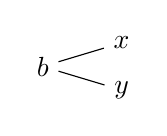
\begin{tikzpicture}[baseline={(0.base)}]
    \node (0) {$b$};
    \node at (1,0.3) (1) {$x$};
    \node at (1,-0.3) (2) {$y$};
    \draw (0) -- (1);
    \draw (0) -- (2);
  \end{tikzpicture}
\]

It properly reflects that \hsinl{x} is never called together with \hsinl{y}.
The analysis then makes use of that information when handling the \hsinl{let} expression binding \hsinl{y}, by effectively performing substitution of the co-call graph of its bound expression (which contains the single node \hsinl{x} without any edges) for \hsinl{y} in the above co-call graph of the body.

After this substitution step, there will be no loop on \hsinl{x}, because there was no edge between \hsinl{y} and \hsinl{x}.
This represents the fact that \hsinl{x} is not called with itself, or only called once, plainly speaking.

Co-call graphs and this rather involved substitution procedure are illuminated in detail in \cref{sec:graph} and \cref{sec:let}.
\Cref{sec:bench} discusses the impact of co-call graphs on analysis precision and performance.

\section{Demand Analyser}\label{sec:dmd}

GHC's approach to strictness and usage analysis is that of \emph{demand analysis}.

It is what we referred to as a cardinality analysis (\cref{sec:card}), integrating both \MinCard and \MaxCard analyses.
To make matters more confusing, the part concerning usage analysis is introduced in \textcite{card}, titled `Modular, Higher-order Cardinality Analysis in Theory and Practice'.
Later chapters refer to the usage analysis as implemented in GHC's Demand Analyser as Cardinality Analysis in title case, to disambiguate it from the notion of cardinality anaysis in \cref{sec:card}.

On top of producing cardinality results, the Demand Analyser also performs \emph{constructed product result analysis} (CPR) \parencite{cpr}. 
The details are irrelevant to this work, but it deserves mention as we will see later.

\subsection{Implementation}

Like Call Arity, the Demand Analyser works by abstract interpretation.
The abstract domain is however quite different from that of CallArity:
It is a product lattice of strictness and usage information (\eg lower and upper bounds of cardinalities).

We focus on the usage analysis (Cardinality Analysis) here, which aims to identify single-entry thunks, one-shot lambdas and absent bindings \parencite[section~2]{card} for the reasons we explained in \cref{sec:card}.
They achieve remarkable precision by a number of interesting features, which describe not only the maximum cardinality of a binding, but also \emph{how} a syntactic thing was used.
We borrow the same language for our usage analysis, so the curious reader can refer to \cref{sec:dom} for a formal definition.

\subsubsection{Call Uses}

Identifying one-shot lambdas requires to know about how the expression containing the lambda was used and to track that information somehow.

The analysis captures this information in \emph{call uses} it tracks in addition to evaluation cardinality.

Consider the following expression, similar to earlier examples:
\begin{haskellcode}
  let f x y = ...
  in f 1 2 + f 1 3
\end{haskellcode}

Here, \hsinl{f} is called twice and while the outer lambda (which binds \hsinl{x}) is not one-shot, the inner lambda is.
Cardinality Analysis expresses that as a call usage of $\omega*C^\omega(C^1(U))$ on \hsinl{f}, where the outer $\omega$ is the evaluation cardinality and the $\omega$ in the superscript of the first $C$ indicates that the outer lambda is not one-shot.
The inner lambda is identified as one-shot, as evident by the superscript $1$ on the inner $C$.

Call uses enable the analysis to differentiate the converse case, where the outer lambda is one-shot, but the inner is not:
\begin{haskellcode}
  let f x y = ...
  in let g = f 1
     in g 2 + g 3
\end{haskellcode}

This results in a call usage of $1*C^1(C^\omega(U))$, reflecting that \hsinl{f} was only evaluated once, because the partial application bound to \hsinl{g} was shared.

\subsubsection{Product Uses}

Call uses would be enough to identify one-shot lambdas.
Inspired by the preceding absence analysis, \textcite{card} however also introduced \emph{product uses} to track absence of parts of a structure.
This is so that the worker/wrapper transformation can expose specialised calling conventions as an inlinable wrapper function, while the worker itself might not be inlinable for different reasons.

Consider the following \hsinl{funny} function:
\begin{haskellcode}
  funny p@(a, b) = sum [1..a]
\end{haskellcode}

Obviously, \hsinl{funny} doesn't use the second component of its pair argument when called.
In terms of the abstract domain, \hsinl{p} is exposed to usage $1*U(1*U, A)$, \eg first evaluated to WHNF and then its first component is used once according to $1*U$, but its second component is absent, $A$.

A neat side-effect of borrowing this from the prior absence analysis is that this is able to capture call uses on type class methods.

\subsubsection{Usage Signatures}

There is another important ingredient to Cardinality Analysis.

Languages like Haskell make it easy to define many small functions, which effortlessly compose to model more complex logic.
This becomes a burden for the compiler, as every analysis heavily relies on the inliner for good interprocedural results.
Even if the inliner does a good job, there are cases where inlining isn't possible for reasons of code size or recursion.

In these cases, an analysis must provide its own interprocedural mechanism to achieve good results.
Cardinality Analysis is no different, so it approximates usage behavior of functions through \emph{usage signatures}.

As always, an example helps to get the point:
\begin{haskellcode}
  let const a b = a
  in const True (fac 1000) 
\end{haskellcode}

In this snippet, \hsinl{const} has a usage signature of $1*U \to A \to \bullet$, meaning that when called with two arguments, \hsinl{const} will use its first argument once, but its second argument not at all.

This is valuable information at the call site of \hsinl{const}, where the expression \hsinl{fac 1000} can be regarded as absent.

In order to have the usage signature for functions available at call sites, Cardinality Analysis analyses the function bound to \hsinl{const} before it analyses the body of the \hsinl{let}.
This \letdnsc rule \parencite{card} is in contrast to Call Arity, where arity information dictates an information flow from the bottom up.

\subsubsection{Thunks}

The \letdnsc approach works quite well for functions.
Things look different for thunks, though:
\begin{haskellcode}
  let x = ...
  in let y = 2*x
     in y + y
\end{haskellcode}

Unleashing \hsinl{y}'s \emph{usage type}, comprised of free variable usages and usage signature, at the evalation sites \letdnsc-style suggests that \hsinl{x} is evaluated twice.
That is not the case, because the reduction to WHNF of \hsinl{y}'s bound expression will be shared, thus \hsinl{x} is actually single-entry.

In order not to lose precision, thunks are analysed after the usage they are exposed to is collected from analysing the body of the binding \hsinl{let} expression.
This bottom-up approach is backwards compared to how functions are treated (\eg bound expression before body) and is embodied in the \letupsc rule.
Call Arity uses an \letupsc-style approach for all bindings, because it isn't concerned with unleashing usage signatures at call sites.

\subsection{Untangling Analyses}\label{sec:untangle}

Demand Analysis as implemented in GHC integrates three interdependent analyses.
We will attempt to provide insight into how information flows between strictness, usage and constructed product result analysis, as well as which other parts of the compiler depend on the produced information.

\begin{figure}[h]
  \centering
  \begin{tikzpicture}[shorten >=1pt,x=10em,y=5em,auto]
    \tikzset{every loop/.style={looseness=4}}
    \tikzstyle{a}=[draw,shape=ellipse]
    \tikzstyle{t}=[draw,shape=rectangle]
    \node (usage) at (0,1) [a] {Usage};
    \node (strict) at (1,1) [a] {Strictness};
    \node (cpr) at (2,1) [a] {CPR};
    \node (ww) at (1,0) [t] {Worker/Wrapper};
    \node (simp) at (1,2) [t] {Simplifier};
    \node (prep) at (0,2) [t] {CorePrep};
    \path[dashed,->,line width=1pt] 
      (usage) edge node {} (strict);
    \path[->,line width=1pt] 
      (usage) edge node[left] {absence} (ww)
      (usage) edge node {one-shot} (simp)
      (usage) edge node {single-entry} (prep)
      (strict) edge node {} (cpr)
      (strict) edge node {} (ww)
      (strict) edge node {} (simp)
      (cpr) edge node {} (ww);
  \end{tikzpicture}
  \caption{Information flow between usage, strictness and constructed product results analysis and how their results are used by different transformations within GHC.}
  \label{fig:dmd}
\end{figure}

\Cref{fig:dmd} references the three analyses in question as well as the transformations which access the analysis results.

Usage analysis, as this thesis will prove, is pretty much a stand-alone analysis; we only rely on arity results from a prior arity analysis (part of GHC's simplifier) to be present to distinguish thunks (which have arity zero) from functions.

The dashed line between usage analysis and strictness analysis indicates that there probably is some kind of information flow, like in the form of absence information. 
It is hard to tell, because the interactions between usage and strictness lattice in \texttt{utils/Demand.hs} are quite convoluted.

Other than that, constructed product result analysis relies on strictness results to be present, as can be reproduced by following the GHC Note\footnote{Notes are a documentation idiom in widespread use within GHC, to be able to refer to explanations by a title and reduce duplicate inline documentation.} `CPR Example' in \texttt{stranal/DmdAnal.hs}.

Absence, strictness and constructed product results are the key ingredients for the worker/wrapper transformation \parencite{ww}.
GHC's simplifier uses one-shot annotations on lambdas for a multitude of optimisations outlined earlier in \cref{sec:usage}.
Single-entry annotations are only exploited by the backend, after the Core-to-Core-pipeline, which is represented by the CorePrep pass in \cref{fig:dmd}.\medskip

We initially tried to integrate Call Arity into the Demand Analyser, but quickly gave up on the endeavor.
Changing the Demand Analyser has far-reaching consequences through the whole compiler and we were afraid to spend more time fixing regressions than to actually solve the core problems of this thesis outlined in the introduction.

In fact, we advocate splitting up the Demand Analyser in its three subanalyses for the following reasons:
\begin{description}
  \item[Complexity] 
    Stricter separation of concerns would definitely get rid of some of the complexity in demand analysis.
    Over the years, many hacks accumulated within the implementation and the intertwining means that it is not always obvious which sub analysis is affected by them.
    The constant context switching is also very distracting.
    Also, \texttt{utils/Demand.hs}, which models the analysis domain, has grown quite big and complex over time.
  \item[Incompatibilities]
    There are a number of hacks to make the analyses work together.

    For example, there is an extra `virgin' iteration only to have stable strictness results available to do CPR analysis (For further details see the Note `Optimistic CPR in the "virgin" case' in \texttt{stranal/DmdAnal.hs}).

    Also the \letupsc rule is a misfit for strictness analysis.
    Strictness does not try to separate `evaluated at least once' from `evaluated multiple times` (\eg $[1,\omega]$ vs. $[\omega,\omega]$), hence accounting for thunk sharing is not needed.
    As we will see later in \cref{sec:let}, \letdnsc provides strictly better precision in some cases (Note `Aggregated demand for cardinality'), so this is unfortunate.
\end{description}

There's also the issue of perfomance:
The Demand Analyser always computes all analysis results, even if only results of one subanalysis might be needed.
On the other hand, the repeated AST traversals if the analysis would be split up probably incur a greater performance hit than what can be gained by being able to analyse more fine-grained.
Of course, this is all just hand-waving as long as there are no measurements.

The combination of these problems lead us to carve out a standalone usage analysis that also generalises the results of Call Arity.
